\documentclass[12pt]{article}
\usepackage{graphicx}
\usepackage{pdfpages}
\graphicspath{ {./figures/} }
\title{Neuroevolution of Task Specialisation in Multi-Agent Systems}
\author{Mostafa Rizk}

\setlength{\parindent}{0pt}

\begin{document}

\maketitle

\section{Introduction}

\subsection{Background \& Motivation}

Multi-agent teams can be used to solve a diverse range of problems such as foraging, collective construction, area coverage and collective manipulation \cite{hamann:Springer:2018,bayindir:neuro:2016,brambilla:SI:2013}.
This research focuses on foraging, when a group of agents must locate and transport resources from one location to another \cite{hamann:Springer:2018,bayindir:neuro:2016,brambilla:SI:2013}, usually a base or nest.
Foraging is of particular interest because it has many real-world analogs, especially in robotics, such as search and rescue \cite{hamann:Springer:2018,bayindir:neuro:2016,brambilla:SI:2013, khamis:Springer:2015}, humanitarian demining \cite{bayindir:neuro:2016,brambilla:SI:2013, khamis:Springer:2015}, hazardous waste cleanup \cite{bayindir:neuro:2016} or planetary exploration \cite{bayindir:neuro:2016}. 
Multi-agent foraging is advantageous over single-agent foraging because agents can improve team performance by working in parallel \cite{khamis:Springer:2015, ericksen:SSCI:2017} or by cooperating and specialising in different sub-tasks \cite{ferrante:PLOS_CB:2015, pini:Swarm_Intelligence:2011, pini:ICSI:2012}, which promises even greater performance.\\

Learning multiple agent policies that collectively achieve a team objective is challenging, however \cite{trianni:SCI:2008,francesca:SI:2014}.
Neuroevolution is a promising technique to address this challenge that applies evolutionary algorithms to neural networks to learn policies \cite{stanley:Nature:2019} .
Neural networks have shown state of the art performance in several domains \cite{marcus:arXiv:2018:deep}, including on agent-based problems \cite{marcus:arXiv:2018:innateness}, in part due to their high representational power \cite{such:arXiv:2017}.
Rather than mapping an action to each individual state, like Q-tables, neural networks are able to generalise, making problems with large state spaces much more feasible to solve \cite{such:arXiv:2017}.
Evolutionary algorithms have also had much success, showing comparable or superior performance to state of the art reinforcement learning algorithms \cite{such:arXiv:2017, salimans:arXiv:2017}.
Neuroevolution has the additonal benefit of being highly parallelisable \cite{salimans:arXiv:2017} and introduces the possibility of using techniques from the literature such as novelty search \cite{lehman:Springer:2011, gomes:SI:2013, gomes:EC:2017}, architecture search \cite{elsken:arXiv:2018, wistuba:arXiv:2019} and others to solve more challenging problems \cite{stanley:Nature:2019}.\\

Evolving specialisation has only been done in a few studies \cite{ferrante:PLOS_CB:2015, nitschke:SEC:2012}, though, with most studies opting for less automated approaches \cite{hamann:Springer:2018}.
While these studies evolved specialisation successfully, their results are difficult to reproduce and it is not clear what the core challenges of evolving specialisation are.
Understanding these challenges can make it easier for future research to produce specialisation, leverage it for foraging and extend it to other multi-agent tasks.

\subsection{Research Questions}

To better understand how specialisation can be evolved, I investigate the following research question:\\

\textbf{How can effective task specialisation be evolved for multi-agent foraging?}\\

To answer this question, I use an experimental framework based on the slope foraging problem used in \cite{ferrante:PLOS_CB:2015} and similar also to \cite{pini:ICSI:2012, pini:Swarm_Intelligence:2011}.
In this problem, a team of agents must retrieve resources from a source location to a nest.
The source is located at the top of a slope and the nest is located at the bottom.
Agents can employ a generalist strategy where they go up the slope, pick up the resource, carry it to the nest and deposit it.
Agents can alternatively employ a specialist strategy where they cooperate with their team-mates.
In the specialist strategy some agents are droppers, who go up to the source and drop resources that fall just short of the nest in an area called the cache, and some agents are collectors, who retrieve resources from the cache and deposit them at the nest.
In \cite{pini:ICSI:2012, pini:Swarm_Intelligence:2011,ferrante:PLOS_CB:2015}, specialist teams are shown to score higher than generalists because they take advantage of a quick transportation method (i.e. dropping down the slope rather than carrying).
I use the slope foraging problem as a test-bed to explore the evolution of specialisation.\\

I look at three key areas to answer the main research question: the fitness landscape of task specialisation problems, centralised vs decentralised approaches to evolution and theoretical modelling of specialisation.
These three areas are explored through the following three sub-questions:\\

\begin{description}
\item[1] \textbf{What are the fundamental features of the fitness landscape of a task specialisation problem?}\\

Neuroevolution is, fundamentally, an optimisation technique that traverses a landscape and depending on the features of the landscape, different algorithms may be successful.
For example, landscapes with a smooth gradient benefit from gradient-based approaches while landscapes with no gradient or multiple optima benefit instead from population-based methods or methods that reward diversity or are more exploratory \cite{oller:AAMAS:2020}.
Knowing what these features are for a specialisation problem informs what algorithms researchers can use to traverse the landscape and achieve specialisation.

\item[2] \textbf{When do centralised and decentralised solutions outperform one another in task specialisation problems?}\\

Key to the problem of evolving specialised cooperative teams is the question of centralised vs decentralised evolution \cite{panait:AAMAS:2005}.
Centralised evolution uses one evolutionary process to evolve a solution for the entire team \cite{panait:AAMAS:2005}.
Decentralised evolution (cooperative coevolution) uses multiple concurrent evolutionary processes, where each process evolves the solution for an individual agent at the same time as the others are evolving \cite{panait:AAMAS:2005}.
Centralised vs decentralised evolution is explained in more detail in Section \ref{learning} of the Appendix.\\

Centralised techniques, theoretically, should be better at finding the best team solution i.e. the team that cooperates most efficiently, but these techniques may not scale with team size because the solution space grows very quickly \cite{panait:AAMAS:2005}.
Additionally, teams evolved using this approach may not be robust to changes in the individual team members; that is, their cooperative strategy will not work if one of the cooperators is replaced \cite{panait:AAMAS:2005}.\\

Decentralised techniques should scale well because each evolutionary process is only looking for a single agent's solution, regardless of the size of the team, so the solution space does not change \cite{panait:AAMAS:2005}.
These techniques should also be robust because throughout each agent's evolutionary process, it never knows what other agents it will be paired with, so the evolved solution should work well regardless of what the other agents on the team do \cite{panait:AAMAS:2005}.\\

Previous works suggests that a decentralised approach is favourable when seeking robustness whereas a centralised one is favourable when seeking cooperation \cite{wiegand:GECCO:2006}, but a thorough analysis has yet to be performed. 
Moreover, the question of how centralised and decentralised systems compare in general, is still an open one \cite{vanLon:AAMAS:2017}.
An empirical comparison of these two approaches in terms of scalability, robustness and degree of specialisation can help determine when it might be preferable to use each approach.

\item[3] \textbf{What is the price of anarchy in task specialisation problems?}\\

While empirical results are valuable, having a theoretical understanding of them helps to generalise findings.
A theoretical model helps interpret results while the results help to refine the model.
Evolutionary game theory is commonly used as a modelling tool in the multi-agent domain \cite{panait:AAMAS:2005, wiegand:GECCO:2006, lanctot:NeurIPS:2017} and provides two useful measures that complement the other two focuses of this research: nash equilibria \cite{hofbauer:BAMS:2003} and the price of anarchy \cite{koutsoupias:ASTACS:1999}.
A Nash equilibrium is a set of strategies, for all players in game, such that no player has an incentive to unilaterally deviate.
If the task specialisation problem is formulated as a game, we can expect the Nash equilibria of that game to correlate to the optima in the fitness landscape.
This is valuable because the landscape of future specialisation problems can be predicted if they have the same features as a particular game/games.
The landscape analysis alone only tells the features of this particular implementation of the task specialisation problem.
The landscape analysis paired with the game theoretic model explaining it, tells the features of other instances of the specialisation problem.\\

The price of anarchy is a measure of how the performance of a socially optimal system, designed by a benevolent dictator, deteriorates when agents can act autonomously to serve their individual interests.
The socially optimal system can be considered analogous to a centralised solution and a system of self-interested agents can be considered analogous to a decentralised solution.
If the price of anarchy matches what is observed in the empirical setup, it supports the conclusion that these results will follow for other instances of the task specialisation problem.
If the price of anarchy does not match, but the model is a correct representation of the problem, then it suggests there are practical issues with implementation that cause a discrepancy.

\end{description}

\section{Landscape Analysis}\label{landscape_analysis}

\textbf{What are the fundamental features of the fitness landscape of a task specialisation problem?}\\

To answer this question, I perform RWG analysis, as proposed in \cite{oller:AAMAS:2020}, to understand the fitness landscape independently of the architecture used to represent agent policies.
This involves randomly sampling several thousand genomes, where each genome represents the neural networks of a team of two agents, evaluating that team over multiple episodes and visualising the distribution of team scores. 
I can then make inferences about things like the gradient of the landscape and the presence of local optima.
Paired with information about each solution's degree of specialisation, I can also make conclusions about how common specialisation is in the landscape and how it correlates to solution quality.\\

I also use dimensionality reduction to reduce the high-dimensional landscape to a 2D representation that maintains the distances between solutions.
This visualisation allows me to make further inferences about the gradient of the landscape and presence of local optima.
But it also makes it possible to infer the number of optima and where specialised and/or high-quality solutions are in the landscape relative to non-specialised and/or low-quality solutions.\\

\subsection{Creating a Fitness Gradient}

One conclusion of the research so far has been that the landscape of task specialisation problems appears to be very flat and thus difficult to find any solution at all, let alone a specialised one.
If a flat fitness landscape is inherent to task specialisation problems, then this is significant because it implies that algorithms that are highly exploratory should be used, as they are with similar problems \cite{oller:AAMAS:2020}.
However, it is also possible that the fitness function might be making evolution unnecessarily difficult because it only rewards task completion, treating partial success the same as failure.
If partial successes are rewarded, the landscape could have a smoother gradient, making it easier for evolution to traverse.
This leads to the following hypothesis:\\

\textbf{Hypothesis 1.1:} Rewarding agents for partial retrieval of the resource will create a smoother fitness gradient.\\

I conducted an experiment to test this hypothesis where I repeated the landscape analysis but with rewards for partial task completion.
The results showed that partial rewards do indeed create a slight gradient but the landscape is still overwhelmingly flat due to a common problem in the literature known as the bootstrapping problem, so the hypothesis is rejected.
Section \ref{smooth_fitness} of the appendix describes the details and results of this experiment and concludes in the discussion that the most appropriate way to address the bootstrapping problem, for this research, is to use the best solution found by RWG as a starting point for evolution, rather than reward partial task completion. 
This avoids the injection of human bias into the search process and makes the conclusions generalisable to more difficult problem instances.

\subsection{Visualising Specialisation}\label{visualising_specialisation}

I already performed the initial analysis of the landscape (Figure \ref{fig:sparse}), however, the visualisation did not contain any information about how specialised each team was i.e. was a given solution a pair of generalists or a pair of specialists? 
Are the better solutions in the landscape usually specialists? 
To visualise this information I need a way of measuring the degree of specialisation of a solution, so the second task in this group is to evaluate some candidate metrics and the third is to incorporate the chosen metric into the landscape analysis.
The hypothesis and experiment are:\\

\textbf{Hypothesis 1.2:} Specialist solutions outperform generalist ones.\\

\textbf{Experiment 1.2- Specialisation Plots of RWG Analysis:}  Use the chosen specialisation metric to assess all the solutions found by RWG analysis and incorporate them into the plots.\\

The most specialised solutions are expected to be at the rightmost of the mean plot and above the generalist ones.
If this is the case, then it supports the hypothesis.
If there are generalist solutions that outperform specialist ones, it disproves the hypothesis.

\subsection{Dimensionality Reduction}

The neural networks used to solve the Slope Foraging problem have hundreds of weights, meaning that the fitness landscape has just as many dimensions and is consequently very difficult to visualise.
Reducing the dimensionality of the problem to two or three dimensions makes visualisation possible and gives many valuable insights into the features of the landscape, especially if combined with a specialisation metric.
How far apart are specialist and generalist solutions in the landscape?
How many optima are there?
What trajectory does evolution take through the landscape?
There are many techniques to choose from \cite{veerapen:GPEM:2018} and further consideration is necessary before choosing one, but Sammon mapping \cite{sammon:IEEETR:1969} is currently the preferred method due to its ability to preserve the relative distances between solutions and its use in other agent-based and neuroevolution studies \cite{kim:GECCO:2003, risi:AB:2010}.

The hypothesis is:\\

\textbf{Hypothesis 1.3:} There are two optima in the landscape, one composed of specialist solutions and one composed of mostly generalist solutions. \\

\textbf{Experiment 1.3- Dimensionality Reduction:} Assemble a dataset of solutions, combining some random ones from rwg and some evolved ones.
Apply the chosen dimensionality reduction technique to the dataset.
Use the chosen specialisation metric to plot the degree of specialisation (in addition to the fitness).\\

If there are indeed two optima, then the hypothesis is supported, otherwise it is rejected.
If, additionally, the specialist solutions are fitter than the generalist ones, Hypothesis 1.2 is further supported.\\

I have already implemented a version of this and began getting preliminary results.

\subsection{Analysis of Different Slope Angles}

For the Slope Foraging task, the slope is what provides evolutionary pressure for specialisation to emerge.
Having no slope at all means there should be no benefit from specialisation and no pressure for it to evolve.
Changing the slope angle changes how beneficial specialisation is. 
Experiments so far have only focused on one slope setting, so further experiments are needed to examine an environment with no slope and an environment with intermediate slope.

Thus:\\

\textbf{Hypothesis 1.4.1:} When the slope is flat, there will only be one optima of generalists and no specialist solutions.\\

\textbf{Hypothesis 1.4.2:} An intermediate slope will have two optima (one specialist and one generalist).\\

\textbf{Hypothesis 1.4.3:} The specialist solutions will outscore the generalists, but the disparity will be smaller than the steeper slope setting. \\

\textbf{Experiment 1.4- RWG with Different Slope Angles:} Repeat RWG, as it was done for previous experiments, but with no slope and intermediate slope.
Then perform 30 evolutionary runs, each with a different seed genome and random seed.
Use the generated data to create RWG analysis plots and perform dimensionality reduction.\\

If there are any specialist solutions found for the 0 slope setting or more than one optima, Hypothesis 1.4.1 is rejected, otherwise it is supported.\\

If the intermediate slope setting has more or less than two optima, Hypothesis 1.4.2 is rejected, if it has exactly two, it is supported.
If the two optima for the intermediate setting are both generalist, both specialist or both a mix of the two, Hypothesis 1.4.2 is also rejected.\\

If Hypothesis 1.4.2 is supported and the specialist solutions do not outscore the generalist solutions, Hypothesis 1.4.3 is rejected.
If the specialist solutions outscore the generalist solutions but by a margin that is greater than or approximately equal to the margin for the steep slope, Hypothesis 1.4.3 is rejected.
If the specialist solutions outscore the generalists by a margin significantly less than the steep slope setting, the hypothesis is supported.\\

\subsection{Decentralised Solutions} 

So far, RWG analysis has been performed but only for teams produced by a centralised algorithm.
It is not possible to perform a meaningful RWG analysis for decentralised algorithms because each solution is a single agent.
An individual agent's fitness depends on its team-mates, meaning that the fitness landscape changes and it is not possible to infer its features.
What algorithm should be used to navigate the landscape when using a decentralised approach?\\

One way to gain insight into the fitness landscape for decentralised algorithms is to use dimensionality reduction.
Consider 2-agent teams in the centralised setup.
A solution in the landscape is the genomes of both agents on the team.
Consider now a 2-agent team in the decentralised setup.
Each agent was evolved using a separate evolutionary process and navigated its own fitness landscape.
However, the end result of the decentralised approach is still a team of two agents, albeit two agents evolved individually.
If the genomes of the two agents are concatenated, their team can be plotted in the same landscape as the teams evolved by the centralised approach.
This does not tell us what the landscape is like for each agent during the learning process, but it shows us how the decentralised algorithm navigates the shared fitness landscape compared to the centralised algorithm.
Does the decentralised algorithm ultimately find the same solutions as the centralised one?\\

Since centralised learning is trying to find the best team solution and specialisation is what is best for the team, it should more frequently find specialisation than decentralised learning. 
In decentralised learning, each agent's learning process is trying to find the best solution in an environment where it does not know who it will be partnered with. 
The best solution should therefore be the one that is most secure for an agent regardless of who their partners are, which is a generalist behaviour.
A generalist can get resources on its own and does not need to rely on others.\\

\textbf{Hypothesis 1.5:} Solutions found by the decentralised algorithm will be primarily generalist whereas solutions found by the centralised algorithm will be primarily specialist.\\

\textbf{Experiment 1.5- Decentralised Dimensionality Reduction:} Perform 30 evolutionary runs of the decentralised setup.
Calculate the degree of specialisation of all evolved solutions.
Concatenate the genomes of all individuals on a team and apply dimensionality reduction to the data.
Combine the decentralised data with the centralised data and plot on the same plot.\\

If the majority of solutions found by the decentralised algorithm are not generalists, the hypothesis is rejected.
If the majority of solutions found by the centralised algorithm are not specialists, the hypothesis is also rejected.
Otherwise, the hypothesis is supported.

\section{Centralised vs Decentralised Solutions}\label{centralised_vs_decentralised}

\textbf{When do centralised and decentralised solutions outperform one another in task specialisation problems?}\\

Following from the description of the learning process in Appendix Section \ref{learning} :\\

\subsection{Scalability}

\textbf{Hypothesis 2.1.1:} If evolution is run with larger team sizes, the fitness of centralised solutions will decrease.\\

\textbf{Hypothesis 2.1.2:} If evolution is run with larger team sizes, the fitness of decentralised solutions will decrease less rapidly than centralised solutions\\

\textbf{Hypothesis 2.1.3} If evolution is run with larger team sizes, the centralised approach will find fewer specialists.\\

\textbf{Hypothesis 2.1.4} If evolution is run with larger team sizes, the decentralised approach will find the same number of specialists.\\

For centralised learning, since it is searching for a team solution, the search space grows rapidly as the number of agents increases, so we can expect learning to find worse solutions for larger teams. 
These solutions should be less fit and it can also be expected that it will be more difficult to find specialisation, if those solutions are indeed fitter.
Since the decentralised approach is not expected to find specialisation in the first place, that is expected to continue for larger teams.\\

For decentralised learning, the space of solutions remains the same for each agent, when the team size increases, however, there are more concurrent learning processes. 
An agent’s score depends on many other agents executing unknown strategies in its environment, and all those strategies affect one another, so the increased noise may also make it difficult to find good solutions for larger teams.
The time taken by the evolutionary process is not considered in the comparison.
However, it is worth noting that the decentralised approach will likely have a slower wall-time if the evolutionary processes are not run in parallel, since evolution must be run once for each agent.
Multi-threading should be implemented to avoid this problem otherwise computation time will scale linearly with the number of agents on the team.\\

\textbf{Experiment 2.1- Evolution with Larger Teams:} Do 30 evolutionary runs (centralised and decentralised) for teams of 4, 6, 8 and 10 agents.
Calculate the specialisation of all evolved solutions.
Plot the average fitness per agent and team specialisation for teams in each setup. \\

If the average fitness per agent increases or remains the same for the centralised setup, Hypothesis 2.1.1 is rejected, otherwise it is supported.\\

If the average fitness per agent of decentralised solutions increases, Hypothesis 2.1.2 is rejected, otherwise it is supported.\\

If the centralised solutions contain the same number of specialists (or more) for larger teams, Hypothesis 2.1.3 is rejected, otherwise it is supported.\\

If the decentralised solutions contain significantly more or fewer specialists, Hypothesis 2.1.4 is rejected, otherwise it is supported.\\

\subsection{Robustness}

As stated in Hypothesis 1.5, decentralised learning should find the safest strategy for an agent, i.e. a generalist strategy. This strategy is successful regardless of the strategies of its team-mates. If an agent is evaluated with new team-mates it has never been paired with before, it should still perform reasonably well. \\

Conversely, an agent from the centralised setup is part of a larger solution. It is likely specialised. We can expect that if the agent is paired with new team-mates, the team performance will suffer. 
The hypotheses are as follows:\\

\textbf{Hypothesis 2.2.1:} When evolved teams have team-members replaced, the average fitness per agent decreases for centralised teams.\\

\textbf{Hypothesis 2.2.2:} When evolved teams have team-members replaced, the average fitness per agent decreases for decentralised teams, but by a smaller margin than centralised teams.\\

\textbf{Hypothesis 2.2.3:} When evolved teams have team-members replaced, the team specialisation decreases for centralised teams.\\

\textbf{Hypothesis 2.2.4:} When evolved teams have team-members replaced, the team specialisation remains the same for decentralised teams.\\

\textbf{Experiment 2.2- Changing Team-mates:} Take all 60 evolved 2-agent teams (30 centralised + 30 decentralised).
For each evolved team, replace one agent 4 times: once with a dropper, once with a collector, once with a generalist and once with a stationary agent.
Calculate the average fitness and team specialisation then repeat for the other agent on the team.
That is a total of $2 \times 30 \times 4 \times 2= 480 \mbox{ fitness evaluations}$. 
Create a violin plot for the centralised setup and one for decentralised setup.
Draw one violin for the original team and one for each replacement (a total of five).
The data for each violin includes when each of the two agents was replaced.
The y-axis shows the fitness and the plots also have a colour scale to show the degree of specialisation.\\

If the average fitness of centralised solutions increases or remains the same, Hypothesis 2.2.1 is rejected, otherwise it is supported.\\

If the average fitness of decentralised solutions significantly increases, Hypothesis 2.2.2 is rejected.
If the average fitness of decentralised solutions decreases by a larger margin than the centralised solutions, Hypothesis 2.2.2. is rejected.
Otherwise it is supported.\\

If the team specialisation of the centralised solutions significantly increases or stays the same, Hypothesis 2.2.3 is rejected.
Otherwise it is supported.\\

If the team specialisation of the decentralised solutions significantly increases or decreases, Hypothesis 2.2.4 is rejected.
Otherwise it is supported.\\

\section{Theoretical Modelling}\label{theoretical_model}

\textbf{What is the price of anarchy in task specialisation problems?}\\

Theoretically, centralised learning is equivalent to a benevolent dictator that assigns roles to each agent on the team so that the collective solution is socially optimal. 
Decentralised learning is equivalent to a group of self-interested individuals where each is trying to find what is best for itself and we expect that is less likely to find a socially optimal solution. 
Calculating the price of anarchy lets us determine how far the team performance drops when agents are self-interested, i.e. how much performance should drop when using decentralised as opposed to centralised learning.\\

\textbf{Hypothesis 3.1.1:} The slope foraging problem is a stag hunt with two Nash equilibria, where the payoff-dominant equilibrium is specialist solutions and the risk-dominant is generalist solutions.\\

\textbf{Hypothesis 3.1.2:} Socially optimal teams are more likely to converge to the payoff-dominant Nash equilibrum while the self-interested teams are more likely to converge to the risk-dominant Nash equilibrium.\\

\textbf{Experiment 3.1- Game-theoretic Modelling:} Formulate a game that models the experimental setup. 
Find the nash equilibria and study the learning dynamics.\\

If the game is indeed a stag hunt, i.e it has two Nash equilibria where the payoff-dominant equilibrium corresponds to agents specialising and the risk-dominant equilibrium corresponds to agents defecting and being generalists, then Hypothesis 3.1.1 is supported.
Otherwise it is rejected.\\

If the socially optimal teams converge to the payoff-dominant equilibrium and the self-interested teams converge to the risk-dominant equilibrium, Hypothesis 3.1.2 is supported.
Otherwise it is rejected.\\

\section{Timeline} \label{timeline}

Each group of tasks in this timeline aligns with one of my research questions, with the exception of two.
One group is for this document.
The other group is for my literature review.
For the literature review, I have created a spreadsheet to systematically keep track of the literature and ensure my research is supported by a firm knowledge of the field. 
Throughout the next few months, I will add relevant papers to the spreadsheet as I delve deeper into each research question, doing brief first passes of each to get an overview and deeper second and third passes for any that are especially relevant.\\

\includepdf{refined_timeline.pdf}

\bibliographystyle{ieeetr}
\bibliography{references}

\appendix

\section{The Learning Process}\label{learning}

Here "learning" refers to evolution.\\

Each agent is controlled by its own neural network. 
The network encodes the agent’s behaviour i.e. it encodes a function that maps from local observations to actions. 
The neural network architecture is fixed, but the weights are changed throughout the learning process.\\

\subsection{Centralised}

In the centralised setup, a learning algorithm creates a population of solutions. 
A solution is a sequence of neural network weights for the network of each agent on the team. 
For example, if a network has 50 weights and there are 4 agents, the solution has a length of 200. 
Each part of the solution is assigned to a random agent. 
The agents then carry out several episodes, starting from random positions at the nest each episode and acting for a fixed number of time steps. 
The score is calculated at the end of each episode and it is the sum of rewards for all resources gathered by the team minus the costs paid by all agents. 
The average score over all episodes is calculated and used to create a new population of solutions. 
This repeats until the algorithm terminates.\\

\subsection{Decentralised}

The decentralised setup has changed since the seminar and now uses a technique called cooperative coevolution. 
In cooperative coevolution, rather than one evolutionary process learning a combined solution for the entire team, each agent on the team has its own evolutionary process learning a solution for only itself. 
For example, if there are 4 agents, there are 4 evolutionary processes running concurrently. 
At generation $i$, each of the 4 processes creates a population of solutions for its agent, where a solution is the weights of a single agent’s neural network. 
The score of a solution at generation i is calculated by pairing it with the best solutions from each of the other 3 agents’ evolutionary processes at generation $i-1$. 
The score is for that single agent’s performance; it is the team reward (total resources collected) divided by the number of agents (regardless of their contribution) minus the cost incurred by that particular agent.\\

\subsection{Difference}

The difference between centralised and decentralised is that a centralised algorithm uses one learning process to learn a solution for the entire team whereas the decentralised algorithm uses multiple concurrent learning processes to learn solutions for each agent independently that are then combined. 
Centralised learning rewards the team while decentralised learning rewards the individual.\\

\section{Creating a Fitness Gradient}\label{smooth_fitness}

\textbf{Hypothesis 1.1:} Rewarding agents for partial retrieval of the resource will create a smoother fitness gradient.\\

This hypothesis is answered by conducting the following experiment:\\

\textbf{Experiment 1.1- RWG Analysis with Modified Fitness:}  Modify the fitness function such that agents are rewarded for partially retrieving a resource.
Specifically, divide the reward for retrieving a resource by the length of the arena and give agents part of the reward if they move the resource a single tile closer to the goal.
Then conduct RWG analysis as described in Section \ref{landscape_analysis} and compare the plots to those produced for the original fitness function.\\

If the mean curve of the distribution has a smoother gradient, then the hypothesis is proven.\\

The plots for the original landscape analysis and the analysis with the new fitness function are shown in Figure \ref{fig:sparse} and Figure \ref{fig:incremental} respectively.\\

\begin{figure}[h]
\centering
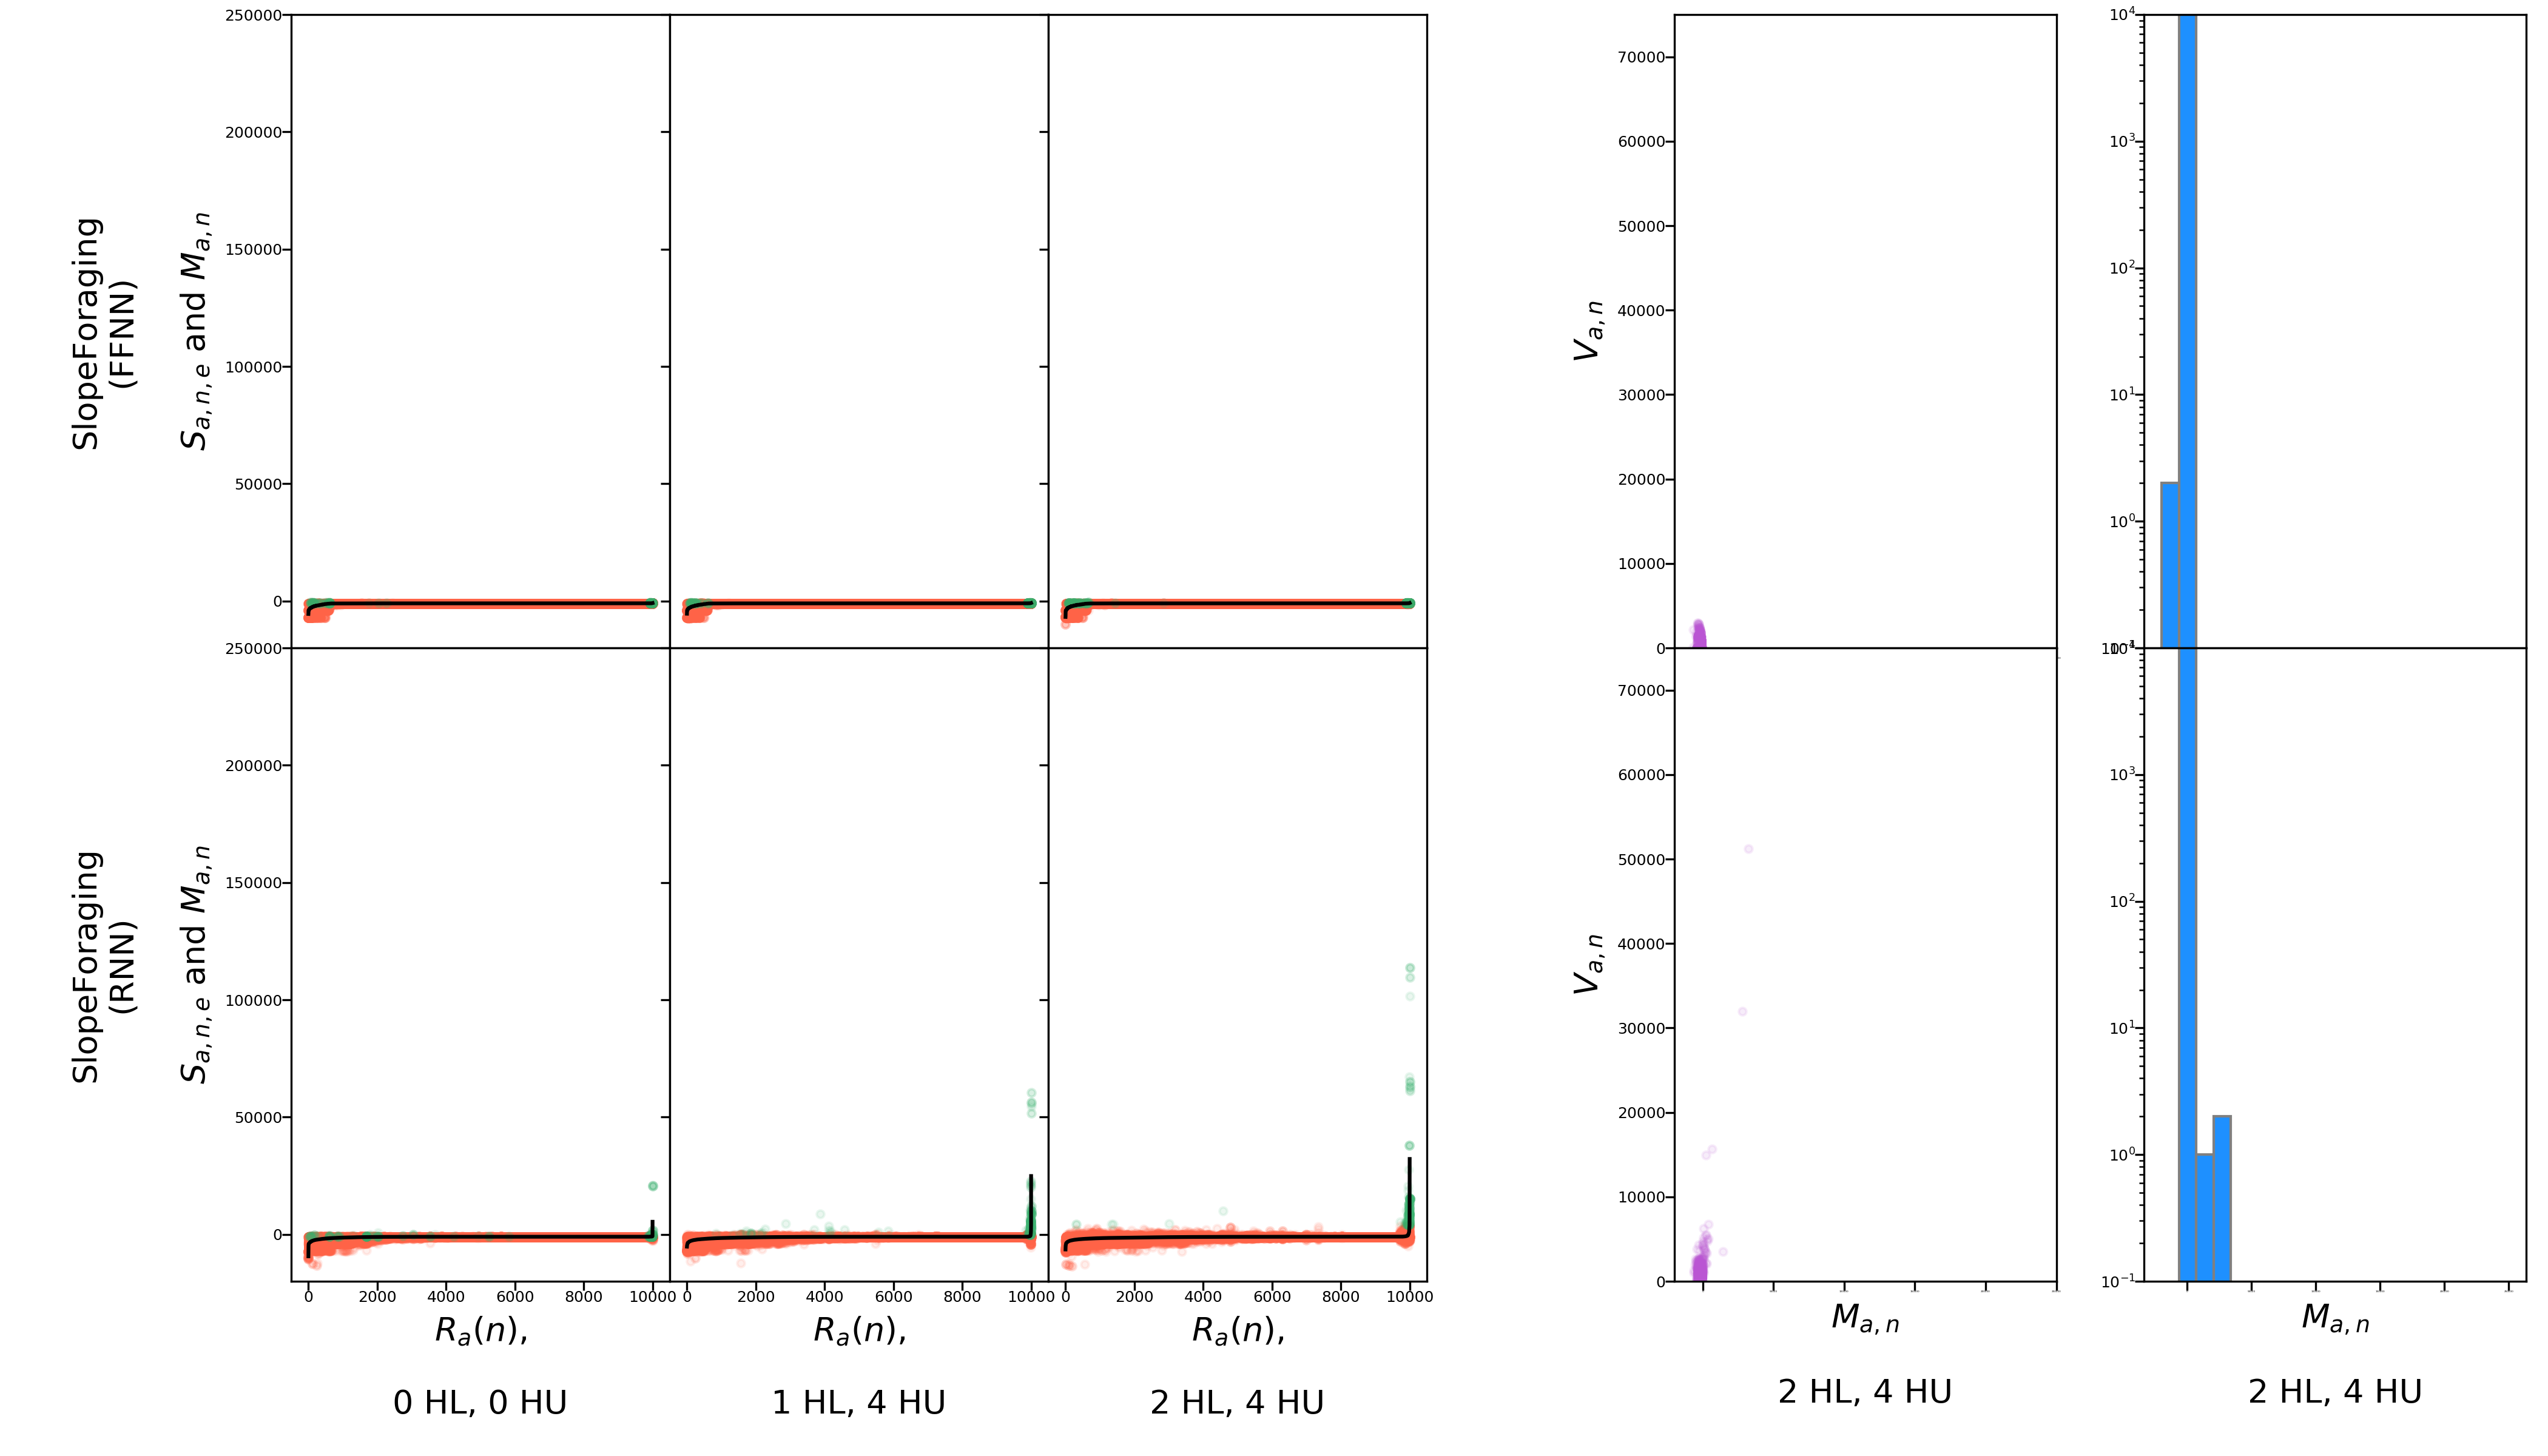
\includegraphics[width=1.0\textwidth]{sparse_rewards.png}
\caption{RWG Analysis with the original fitness function}
\label{fig:sparse}
\end{figure}

\begin{figure}[h]
\centering
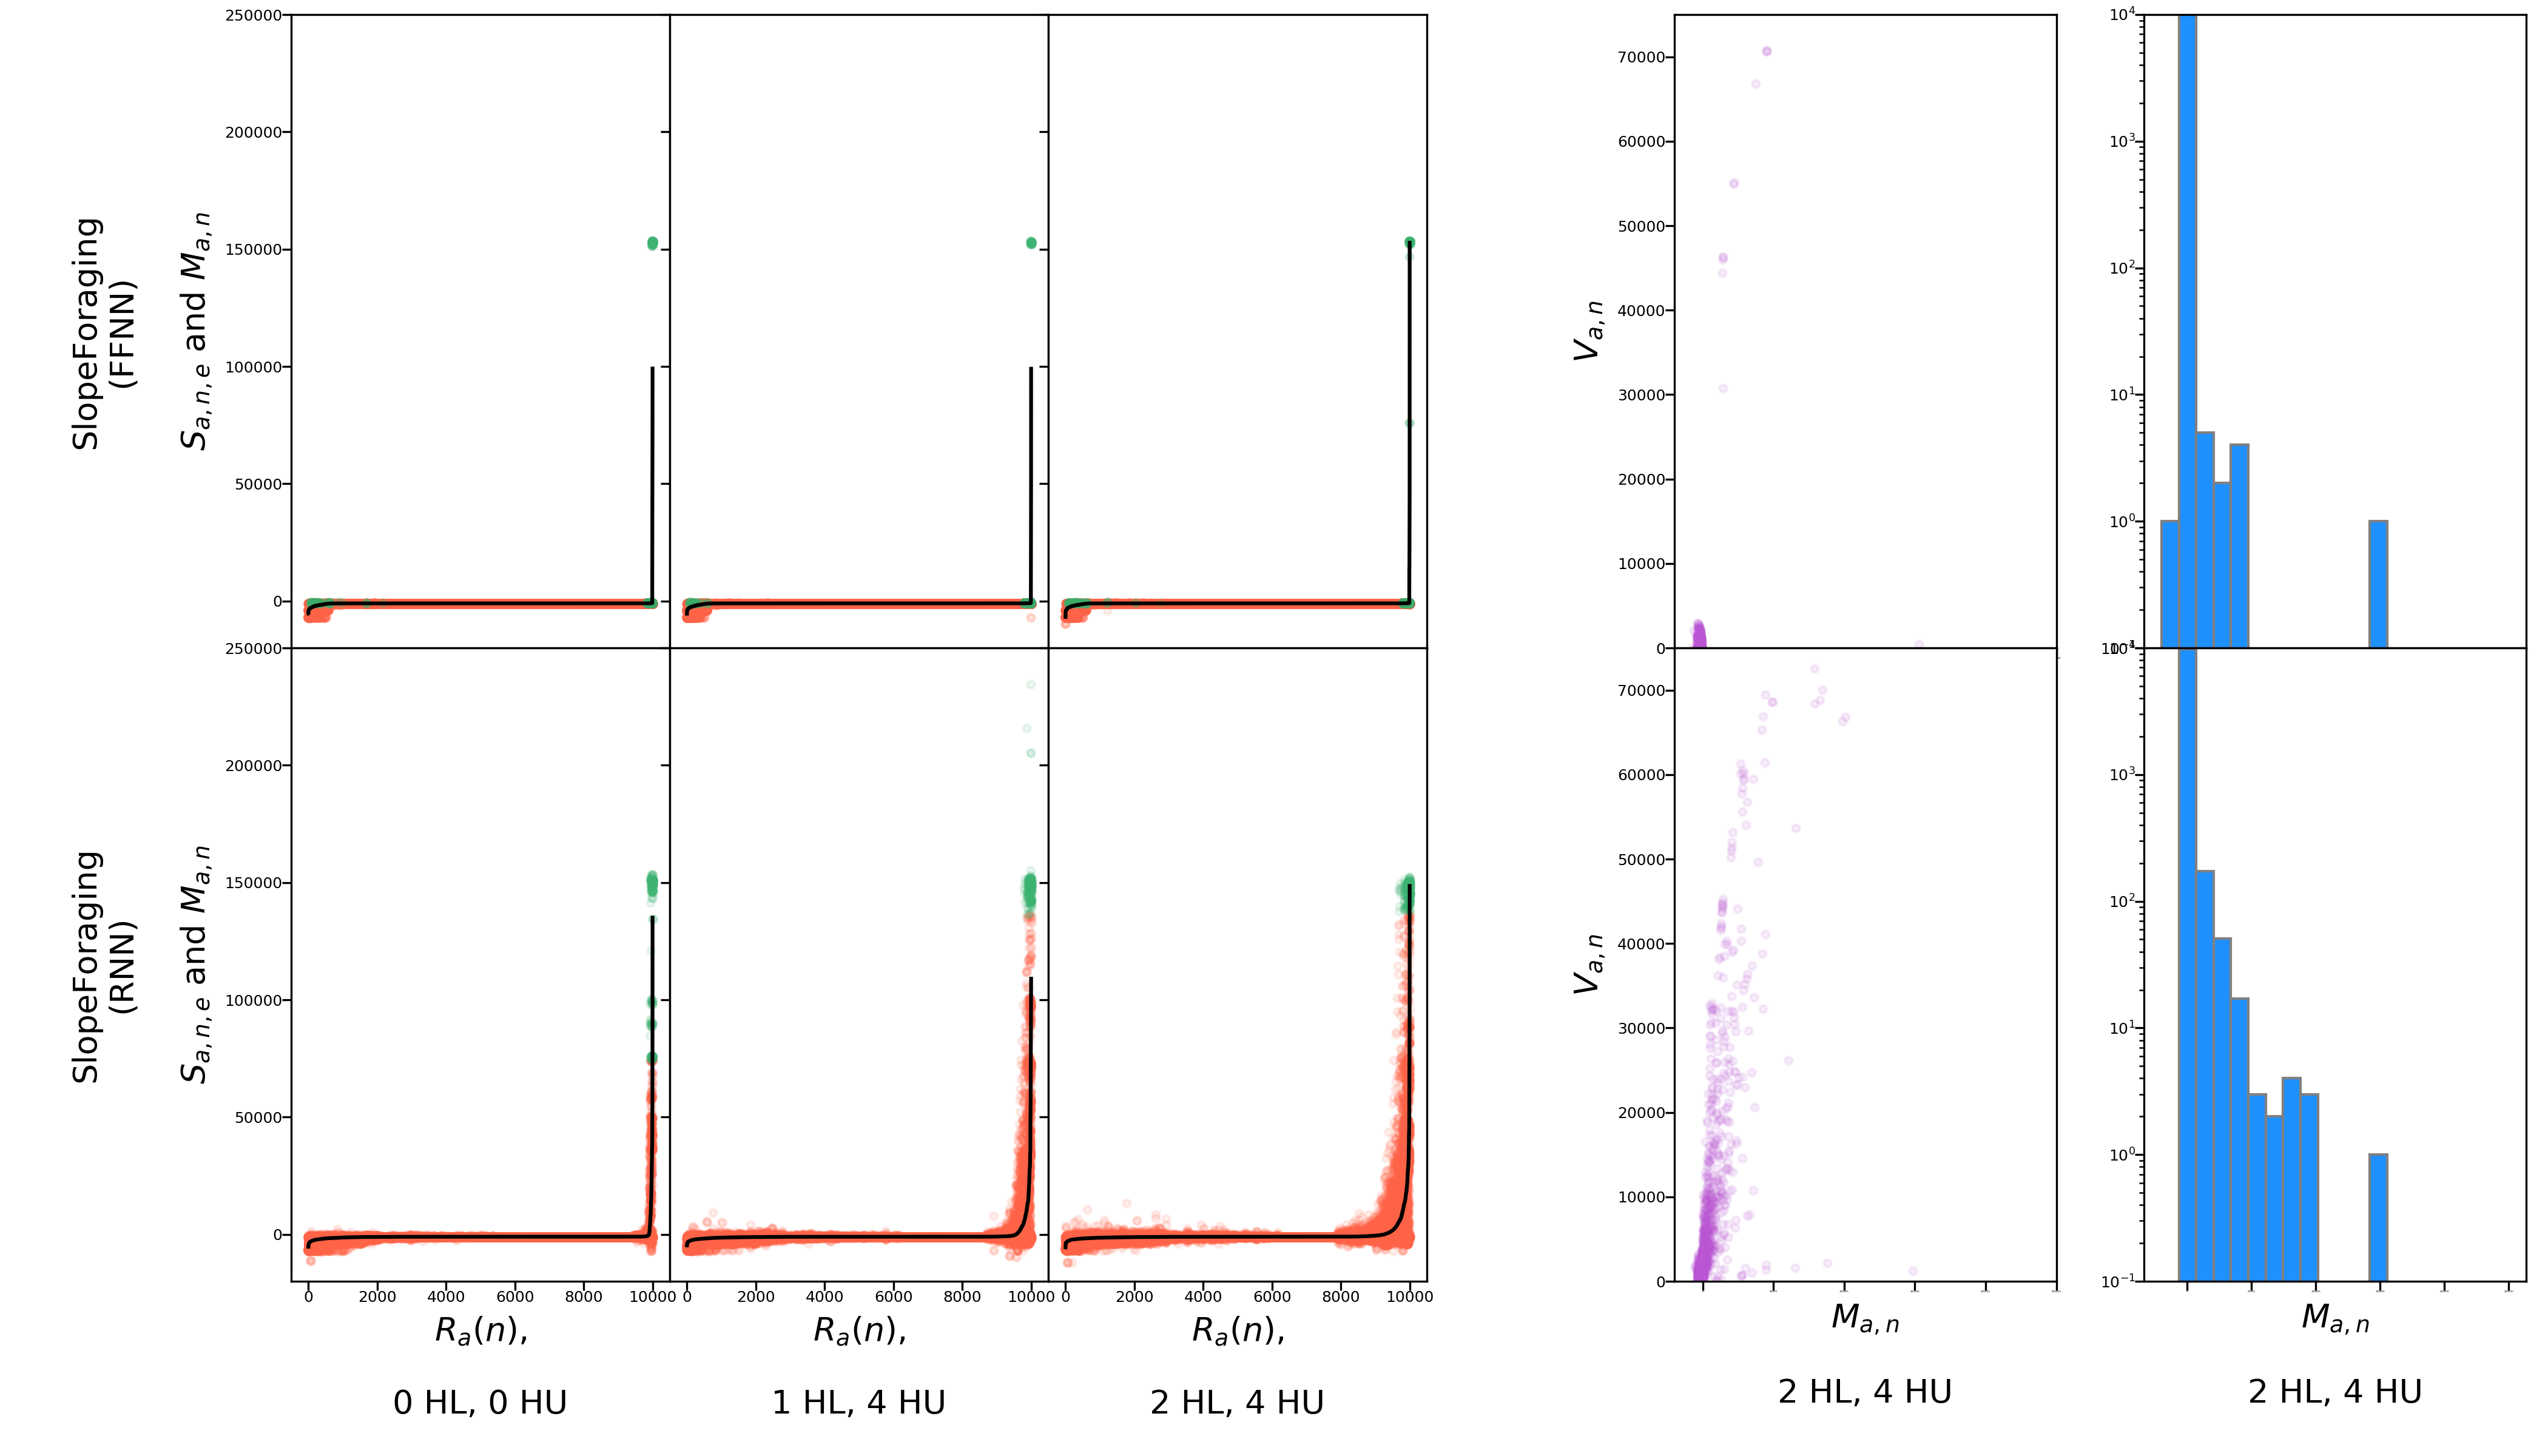
\includegraphics[width=1.0\textwidth]{incremental_rewards.png}
\caption{RWG Analysis with incremental rewards}
\label{fig:incremental}
\end{figure}

Looking at the 6 mean plots in Figure \ref{fig:incremental} compared to Figure \ref{fig:sparse}, we see that with incremental rewards, the solutions do in fact form more of a gradient towards the right end of the plot, in particular for RNNs (bottom row). 
This means that a lot of the solutions in the landscape are partially successful at retrieving resources. 
However, the landscape is still largely flat. 
This is presumably because most solutions in the landscape don't even get to the point of picking up a resource from the source.\\ 

Thus the answer to Hypothesis 1.1 is:\\

\textbf{Answer 1.1:} Rewarding agents for partial retrieval of the resource creates a smoother fitness gradient, but the landscape is still largely flat.\\

In order to further smooth the fitness landscape there would need to be rewards for partial progress up the slope, but the problem with this is that it is likely to disincentivise the collector behaviour in evolution.
Why would an agent stay at the nest and collect resource when they are rewarded for going up the slope? 
Additionally, while this problem is simple enough to smooth the fitness gradient in this way, such smoothing may not be possible for other more complex problems.
The purpose of this research is to understand how to use AI to find good solutions with minimal (if any) human intervention.\\

Moreover, the flatness of the landscape is, to some extent, inherent to this task.
This is a problem common in evolutionary computation known as the bootstrapping problem \cite{Silva:EC:2016, Wei:ALR:2019}.
Bootstrapping is "when the task is too demanding for the fitness function to apply any meaningful selection pressure on a randomly generated population of initial candidate solutions" \cite{Silva:EC:2016}.
The bootstrapping problem often occurs when the goal behaviour is complex relative to the very simple available actions \cite{Wei:ALR:2019}.
For this problem, the available actions are primitives like 'move forward one tile' and 'move backward one tile'.
When putting together sequences of these actions, most sequences will obviously not be very successful.
There are many proposed solutions to solving the bootstrapping problem and they fall under the broad categories of inserting human knowledge into the learning process or increasing the diversity of solutions \cite{Silva:EC:2016}.
Smoothing the landscape falls under the former category, but this family of techniques has some shortcomings, in particular it reduces the potential for automation and risks the experimenter introducing negative biases.
Using rwg to find a seed falls under the second category; it has the shortcoming of additional computation, which may not scale well for problems with larger solution spaces, but for those problems there is a wealth of alternative techniques for increasing diversity, such as novelty search.
In keeping with the spirit of AI, I have chosen to continue using the more challenging fitness function.

\section{List of Hypotheses}

\begin{description}
\item[1] \textbf{What are the fundamental features of the fitness landscape of a task specialisation problem?}\\

\textbf{Hypothesis 1.1:} Rewarding agents for partial retrieval of the resource will create a smoother fitness gradient.\\

\textbf{Hypothesis 1.2:} Specialist solutions outperform generalist ones.\\

\textbf{Hypothesis 1.3:} There are two optima in the landscape, one composed of specialist solutions and one composed of mostly generalist solutions. \\

\textbf{Hypothesis 1.4.1:} When the slope is flat, there will only be one optima of generalists and no specialist solutions.\\

\textbf{Hypothesis 1.4.2:} An intermediate slope will have two optima (one specialist and one generalist).\\

\textbf{Hypothesis 1.4.3:} The specialist solutions will outscore the generalists, but the disparity will be smaller than the steeper slope setting. \\

\textbf{Hypothesis 1.5:} Solutions found by the decentralised algorithm will be primarily generalist whereas solutions found by the centralised algorithm will be primarily specialist.\\

\item[2] \textbf{When do centralised and decentralised solutions outperform one another in task specialisation problems?}\\

\textbf{Hypothesis 2.1.1:} If evolution is run with larger team sizes, the fitness of centralised solutions will decrease.\\

\textbf{Hypothesis 2.1.2:} If evolution is run with larger team sizes, the fitness of decentralised solutions will decrease less rapidly than centralised solutions\\

\textbf{Hypothesis 2.1.3} If evolution is run with larger team sizes, the centralised approach will find fewer specialists.\\

\textbf{Hypothesis 2.1.4} If evolution is run with larger team sizes, the decentralised approach will find the same number of specialists.\\

\textbf{Hypothesis 2.2.1:} When evolved teams have team-members replaced, the average fitness per agent decreases for centralised teams.\\

\textbf{Hypothesis 2.2.2:} When evolved teams have team-members replaced, the average fitness per agent decreases for decentralised teams, but by a smaller margin than centralised teams.\\

\textbf{Hypothesis 2.2.3:} When evolved teams have team-members replaced, the team specialisation decreases for centralised teams.\\

\textbf{Hypothesis 2.2.4:} When evolved teams have team-members replaced, the team specialisation remains the same for decentralised teams.\\

\item[3] \textbf{What is the price of anarchy in task specialisation problems?}\\

\textbf{Hypothesis 3.1.1:} The slope foraging problem is a stag hunt with two Nash equilibria, where the payoff-dominant equilibrium is specialist solutions and the risk-dominant is generalist solutions.\\

\textbf{Hypothesis 3.1.2:} Socially optimal teams are more likely to converge to the payoff-dominant Nash equilibrum while the self-interested teams are more likely to converge to the risk-dominant Nash equilibrium.\\

\end{description}


\section{List of Experiments}
\textbf{Experiment 1.1- RWG Analysis with Modified Fitness:}  Modify the fitness function such that agents are rewarded for partially retrieving a resource.
Specifically, divide the reward for retrieving a resource by the length of the arena and give agents part of the reward if they move the resource a single tile closer to the goal.
Then conduct RWG analysis as described in Section \ref{landscape_analysis} and compare the plots to those produced for the original fitness function.\\

\textbf{Experiment 1.2- Specialisation Plots of RWG Analysis:}  Use the chosen specialisation metric to assess all the solutions found by RWG analysis and incorporate them into the plots.\\

\textbf{Experiment 1.3- Dimensionality Reduction:} Assemble a dataset of solutions, combining some random ones from rwg and some evolved ones.
Apply the chosen dimensionality reduction technique to the dataset.
Use the chosen specialisation metric to plot the degree of specialisation (in addition to the fitness).\\

\textbf{Experiment 1.4- RWG with Different Slope Angles:} Repeat RWG, as it was done for previous experiments, but with no slope and intermediate slope.
Then perform 30 evolutionary runs, each with a different seed genome and random seed.
Use the generated data to create RWG analysis plots and perform dimensionality reduction.\\

\textbf{Experiment 1.5- Decentralised Dimensionality Reduction:} Perform 30 evolutionary runs of the decentralised setup.
Calculate the degree of specialisation of all evolved solutions.
Concatenate the genomes of all individuals on a team and apply dimensionality reduction to the data.
Combine the decentralised data with the centralised data and plot on the same plot.\\

\textbf{Experiment 2.1- Evolution with Larger Teams:} Do 30 evolutionary runs (centralised and decentralised) for teams of 4, 6, 8 and 10 agents.
Calculate the specialisation of all evolved solutions.
Plot the average fitness per agent and team specialisation for teams in each setup. \\

\textbf{Experiment 2.2- Changing Team-mates:} Take all 60 evolved 2-agent teams (30 centralised + 30 decentralised).
For each evolved team, replace one agent 4 times: once with a dropper, once with a collector, once with a generalist and once with a stationary agent.
Calculate the average fitness and team specialisation then repeat for the other agent on the team.
That is a total of $2 \times 30 \times 4 \times 2= 480 \mbox{ fitness evaluations}$. 
Create a violin plot for the centralised setup and one for decentralised setup.
Draw one violin for the original team and one for each replacement (a total of five).
The data for each violin includes when each of the two agents was replaced.
The y-axis shows the fitness and the plots also have a colour scale to show the degree of specialisation.\\

\textbf{Experiment 3.1- Game-theoretic Modelling:} Formulate a game that models the experimental setup. 
Find the nash equilibria and study the learning dynamics.\\
\end{document}
